
\chapter{Делаем Компоненты красивыми}

Наш путь по лучшим практикам и паттернам React пришел к моменту, когда мы хотим сделать наши компоненты красивее. Для этого мы разберемся с вопросом, почему обычный CSS не всегда является наилучшим вариантом для стилизации компонент, и какие есть альтернативы.

Мы начнем со встроенных стилей, библиотеки Radium, CSS модулей и Styled Compopnents, а затем детально разберем волшебство CSS в JavaScript.

Вопрос стилизации в React стоит очень горячо и вызывает множество споров, поэтому эта глава требует непредвзятости и готовности оценить плюсы и минусы различных инструментов.

В этой главе мы рассмотрим следующие вопросы:

\begin{itemize}
	\item Общие проблемы масштабируемости CSS
	\item Встроенные стили в React и их отрицательные стороны
	\item Как библиотека Radium помогает исправить проблемы встроенных стилей
	\item Как настроить проект с нуля для работы с Webpack и CSS Модулей
	\item Возможности CSS Модулей и их преимущества перед глобальными стилями
	\item Современный подход к стилизации компонентов с библиотекой Styled Components
\end{itemize}

\section{CSS in JS}

Многие знают, что для стилизации в React переломный момент произошел в Ноябре 2014 года, когда \textit{Кристофер Шедо (Christopher Chedeau)} выступил на конференции NationJS.

Кристофер, также известный в интернете как \textit{Vjeux}, работает в Facebook и способствует развитию React. На этой конференции он рассказал о проблемах с CSS при масштабировании приложений, которые они встретили в Facebook.

Важно знать об этих проблемах, так как многие из них часто встречаются на практике, а также будет легче понять необходимость разных концепций, таких как \textbf{встроенные стили} и \textbf{локальные классы}.

На слайде вы можете увидеть один из слайдов с этой презентации со списком главных проблем с CSS:

\begin{figure}[hbt]
  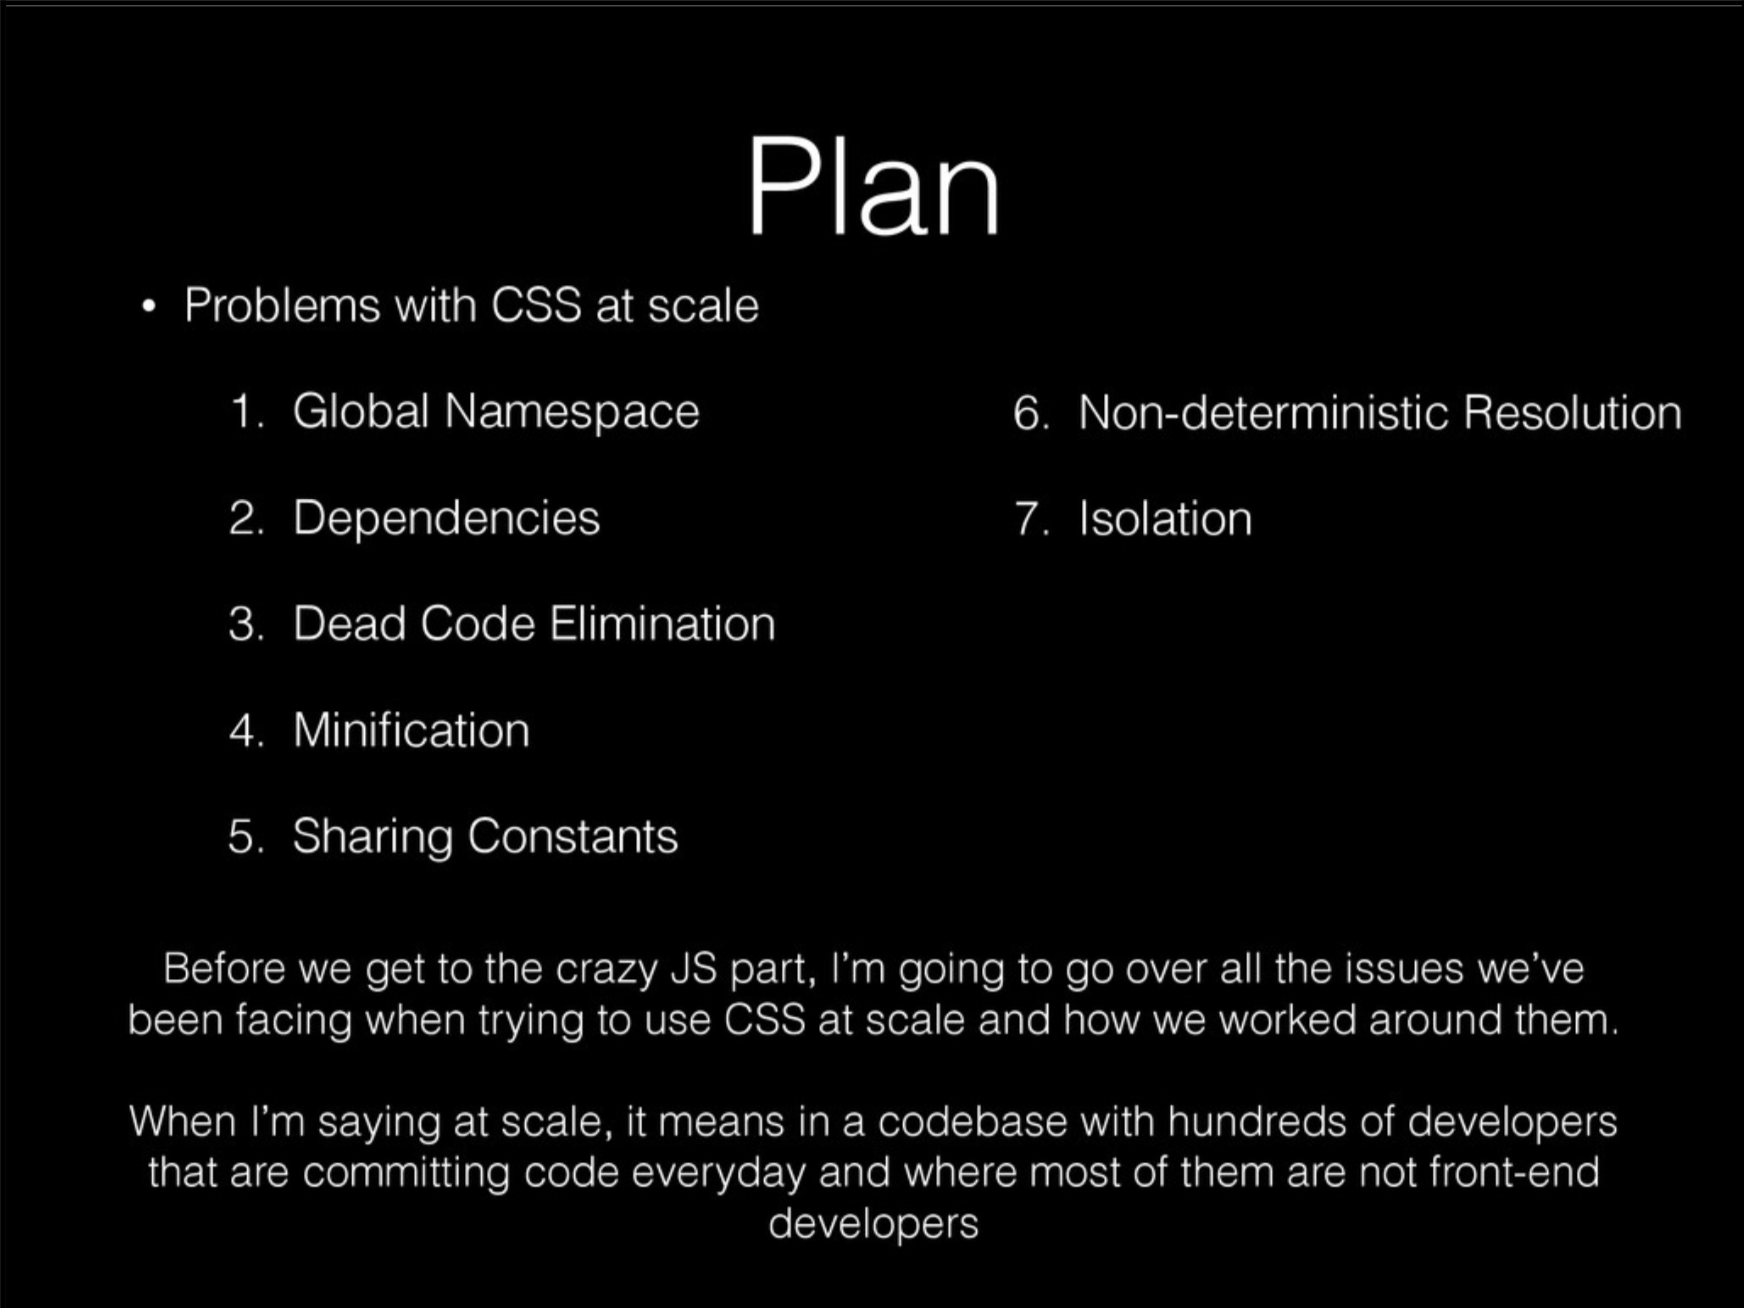
\includegraphics[width=1.\textwidth]{images/css-problems-slide}
\end{figure}

Первая и хорошо известная проблема CSS заключается в глобальных селекторах. Не важно, как вы организовали свой код, использовали ли пространства имен или BEM методологию, в конце все равно стили окажутся в одном глобальном пространстве имен. И это ошибка не только идеологически, это ведет к множеству ошибок и ухудшает поддерживаемость большой кодовой базы. Когда мы работаем в больших командах, не так просто знать о существовании конкретного класса или стилизованного элемента, что ведет к добавлению большего количества классов вместо переиспользования существующих.

Следующая проблема относится к определению зависимостей. На деле бывает очень сложно понять, от каких именно стилей зависит конкретный компонент. Так как стили глобальны, они могут использоваться из любых компонентов, а любой компонент может использовать любые стили. В таких условиях может быть очень легко потерять контроль.

Фронтенд разработчики привыкли использовать препроцессоры для разделения CSS на модули, но в итоге для браузера все равно генерируется большой CSS бандл. Так как объем кода CSS быстро растет, мы получаем еще одну проблему с \textbf{удалением неиспользуемого кода (dead code elimination)}. Так как сложно понять, какой стиль к какому компоненту относится, задача удаления неиспользуемого кода становится еще сложнее. Также, если учесть каскадную природу CSS, удаление любого селектора или правила может привести к непредсказуемым последствиям в браузере.

Минификация селекторов и имен классов также добавляет головной боли и в CSS и в JavaScript приложение. Хотя на первый взгляд эта задача кажется простой, на деле все усложняется, когда классы добавляются во время исполнения программы или высчитываются на клиенте.

Отсутствие возможности минифицировать CSS сильно сказывается на производительности, так как может значительно сказаться на размере CSS файлов.

Также в рамках обычного CSS нетривиально создать константы, общие для CSS и JavaScript. Например для случаев, когда мы хотим знать высоту заголовка, чтобы рассчитать расположение элементов относительно него.

Обычно, JavaScript API используется для получения нужных значений, однако было бы значительно оптимальней использовать общие константы и избежать дорогих вычислений во время исполнения программы. Это и есть пятая проблема, которую Vjeux и другие разработчики Facebook попытались решить.

Шестая проблема заключается в недетерминированный обработке файлов CSS. По факту, в CSS важен порядок обработки файлов с исходниками, поэтому, если файлы грузятся по требованию, то сохранение их порядка не гарантируется, что ведет к применению неверных стилей к компонентам. 

Предположим, что мы хотим оптимизировать загрузку CSS и загружать стили для конкретной страницу только тогда, когда пользователь открывает эту страницу. Если стили, которые относятся к последней странице, содержат правила, которые затрагивают остальное приложение, то отображение всего приложения может измениться. Например, если пользователь вернется по истории к предыдущей странице, она может несколько отличаться от того, что было до этого.

Очень сложно контролировать различные комбинации стилей, правил и путей, но возможность загружать CSS по мере необходимости критична для производительности приложения.

И седьмая проблема, о которой говорит Кристофер Шедо, связана с изоляцией компонент. В CSS очень сложно добиться изоляции файлов или компонентов между собой. Так как селекторы глобальны, они могут быть легко перезаписаны. Это нетривиальная задача, определить финальные стили компонента по примененным к нему классам, так как любой компонент может быть затронут любыми стилями, находящимися в приложении.

Я рекомендую посмотреть это выступление, если вы хотите узнать больше о проблемах масштабируемости CSS. Даже если этот вопрос выглядит сложным и противоречивыми, стоит открыто подходить к нему, чтобы найти решение, которое лучше всего подойдет в вашем случае:

\begin{quotation}
https://vimeo.com/116209150	
\end{quotation}

В заключении этого выступления было сказано, что для решения этих проблем масштабирования CSS в Facebook остановились на использовании \textit{встроенных стилей (inline styles)}.

В следующей части мы рассмотрим, как использовать встроенные стили в React, и какие есть плюсы и минусы у этого подхода.

\section{Встроенные стили}

Документация React советует разработчикам использовать встроенные стили для стилизации компонент. Это выглядит странно, так как за прошедшие годы мы усвоили, что разделение отвественности это хорошо, и мы не должны смешивать разметку и CSS.

React пытается изменить взгляд на разделение ответственности с привычного разделения технологий на разделение компонент. Разделение разметки, стилей и логики на разные файлы, которые сильно связаны и не могут работать по отдельности, иллюзия. Даже если это делает структуру чище, это не приносит реальной выгоды.

В React мы комбинируем компоненты, которые являются базовыми блоками для создания приложения. Мы можем переносить блоки по всему приложению и, независимо от того, где используются компоненты, они должны предоставлять одинаковую логику и отображение.

Это одна из причин, почему объединение стилей с компонентом с помощью встроенных стилей может иметь смысл в React.

Прежде всего посмотрим, как вообще использовать встроенные стили в React компонентах. Создадим кнопку с текстом \textbf{Click me!} и изменим у нее цвета фона и текста:

\begin{lstlisting}
const style = {
  color: 'palevioletred',
  backgroundColor: 'papayawhip',
}

const Button = () => <button style={style}>Click me!</button>
\end{lstlisting}

Как вы видите, использовать встроенные стили очень просто. Нам достаточно создать объект, в котором будут пары ключей и значений как в обычном CSS.

Единственный нюанс, правила с дефисом в названии должны быть записаны в горбатом регистре, а значения передаваться как строки, то есть в кавычках.

Есть несколько отличий при использовании вендорных префиксов. Например, если мы хотим определить переход (transition) в \textbf{webkit}, мы должны использовать атрибут WebkitTransition, который начинается с заглавной буквы. Это правило работает для всех вендорных префиксов кроме \textbf{ms}, которой должен быть в нижнем регистре.

Помимо этого, числа могут использовать без кавычек и единиц измерения, тогда они будут считаться пикселями.

Следующий фрагмент стилей устанавливает высоту в $100px$:

\begin{lstlisting}
const style = {
  height: 100,
}
\end{lstlisting}

Встроенные стили не только прекрасно работают, но и позволяют делать вещи, которые сложно сделать в CSS. Например, мы можем пересчитать значения стилей на клиенте во время исполнения, что мы увидим в следующим примере.

Предположим, что мы хотим создать поле ввода, размер шрифта в котором будет зависеть от его значения. То есть если значение поля будет равно 24, то и размер шрифта должен быть 24 пикселя. Сделать это с помощью CSS невозможно, также нужно приложить значительные усилия, чтобы сделать это в JavaScript.

Посмотрим, как легко сделать это со встроенными стилями.

Нам нужно будет хранить состояние компонента, поэтому создадим для него класс:

\begin{lstlisting}
class FontSize extends React.Component
\end{lstlisting}

В конструкторе класса определим начальное значение компонента, а также привяжем обработчик событий ввода к экземпляру этого класса:

\begin{lstlisting}
constructor(props) {
  super(props)
  
  this.state = {
    value: 16,
  }
  
  this.handleChange = this.handleChange.bind(this)
}
\end{lstlisting}

Мы создадим простой обработчик, который будет только обновлять состояние компонента в соответствии с вводимыми пользователем данными:

\begin{lstlisting}
handleChange({ target }) {
  this.setState({
    value: Number(target.value),
  })
}
\end{lstlisting}

И в конце мы создаем поле ввода с числовым типом, значение которого контролируется нашим компонентом через значение состояния и обработчик событий ввода.

Также мы передадим в атрибут $style$ этого поля ввода объект с актуальным значение размера шрифта. Как говорилось выше название правило должно быть в горбатом регистре, то есть мы должны определить параметр $fontSize$:

\begin{lstlisting}
render() {
  return (
    <input
      type="number"
      value={this.state.value}
      onChange={this.handleChange}
      style={{ fontSize: this.state.value }}
    />
  )
}
\end{lstlisting}

Как мы видим, при изменении значения поля ввода обновляется состояние компонента, что влечет за собой перерисовку компонента. В момент перерисовки значение размера шрифта берется из состояния компонента, которое берется из состояния. Таким образом размер шрифта меняется вслед за значением поля ввода. 

Как и у любого другого решения у встроенных стилей есть свои плюсы и минусы. И в данном случае последних не мало.

Например, со встроенными стилями невозможно использовать псевдоклассы (такие как $:hover$) и псевдоэлементы, что является большим ограничением, если вы хотите создать интерактивный и анимированный UI.

Есть множество костылей (workarounds), которые вы можете использовать для обхода этих ограничений. Например вы можете обычные элементы вместо псевоэлеменов, но для симуляции поведения CSS придется использовать CSS, что не оптимально.

То же самое относится и к \textbf{Медиа запросам (Media queries)}, которые нельзя определить с помощью встроенных стилей, что затрудняет создание адаптивного интерфейса. Также, так как стили передаются через JavaScript объект, во встроенных стилях невозможно использовать style fallbacks:

\begin{lstlisting}
display: -webkit-flex;
display: flex;
\end{lstlisting}

Все из-за того, что JavaScript объекты не могут содержать два атрибута с одинаковым именем. По этой причине использовать style fallbacks невозможно, хотя было бы хорошо иметь возможность их использовать при необходимости.

Еще одна возможность CSS, которую невозможно использовать через встроенные стили, это \textbf{Анимации}. Основной костыль (workaround) в этом случае, определить анимации глобально и использовать их внутри атрибута элементов $style$.

После использования встроенных стилей для предопределения стилей из CSS мы вынуждены использовать ключевое слово $!important$, что является плохой практикой, так как предотвращает применение других стилей к элементу.

И самое ужасное, что происходит при использовании встроенных стилей, это значительное усложнение отладки приложения. Мы вынуждены использовать названия классов для поиска элементов через DevTools браузера в целях отладки и проверки, какие стили были применены.

При использовании встроенных стилей все созданные стили окажутся в атрибуте $tyle$ созданного HTML элемента, что усложняет их отладку.

Например, кнопка из предыдущего примера будет отображена в следующий элемент:

\begin{lstlisting}
<button style="color: palevioletred; background-color: papayawhip;">Click me!</button>
\end{lstlisting}

Один такой такой элемент несложно прочитать, но представьте, что будут сотни таких элементов стилей. В этот момент это начинает превращаться в проблему.

Если вы отлаживаете список таких элементов, в котором у каждого элемента своя копия стилей, то при изменении одного элемента в браузере вы увидите, что меняется только элемент, который вы редактируете, а все соседние элементы остаются неизменными. 

И помимо всего этого, если вы рендерите приложение на стороне сервера (подробнее мы поговорим об этом в Главе 8), то при использовании встроенных стилей размер страницы будет значительно больше. 

Алгоритмы сжатия могут достаточно сильно сжать получившийся HTML, так как в нем будет много повторяющихся частей, в некоторых случаях загрузка критичной части CSS может быть даже хорошей идеей, но в целом мы должны стремиться избежать этого.

Таким образом мы приходим к тому, что встроенные стили создают проблем больше чем решают.

По этим причинам сообщество создало другие инструменты для решения проблем встроенных стилей, не теряя при этом объединения стилей с компонентами. 

После выступления Кристофера Шедо множество разработчиков задумались о проблеме встроенных стилей и начали искать новые решения для использования CSS в JavaScript.

Автор книги изучил все из них и опубликовал репозиторий, в котором создал простую кнопку с помощью каждого из этих методов:

\begin{quotation}
https://github.com/MicheleBertoli/css-in-js
\end{quotation}

В начале их было две или три, но сейчас насчитывается уже больше 40.

В следующих частях мы разберем самые популярные из них.

\section{Radium}

\section{CSS Modules}

\subsection{Webpack}

\subsection{Setting up a project}

\subsection{Locally scoped CSS}

\subsection{Atomic CSS Modules}

\subsection{React CSS Modules}

\section{Styled Components}

\section{Summary}















